
\item Determine a velocidade do bloco $A$ de \SI{30}{\kilogram} se os dois blocos são soltos do repouso e o bloco $B$ de \SI{20}{\kilogram} se desloca \SI{0.6}{\meter} subindo o plano inclinado. O coeficiente de atrito cinético entre ambos os blocos e os planos inclinados é de $\mu_{k}=0.10$.

\import{answers/}{answer-10}

\vspace{-2cm}
\begin{flushright}
    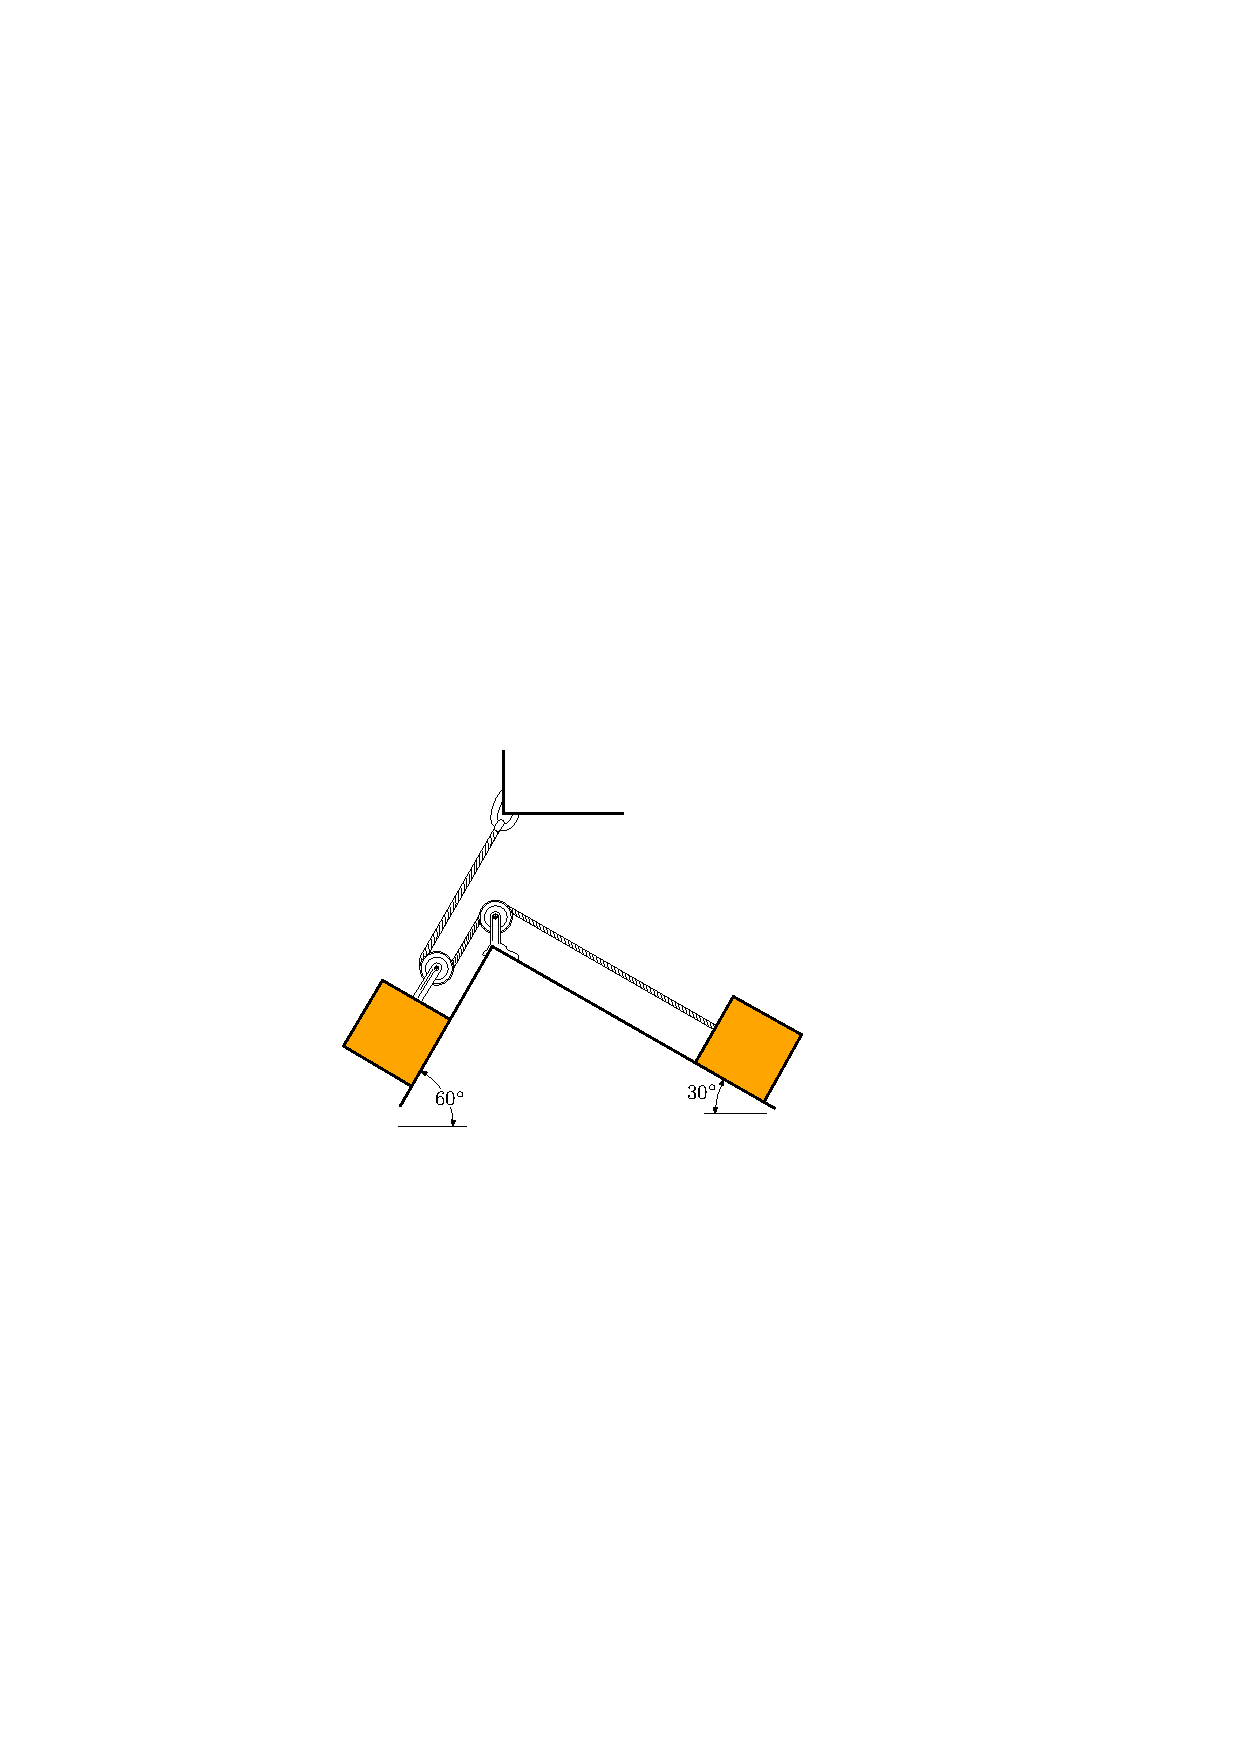
\includegraphics[scale=1.2]{images/draw_10.pdf}
\end{flushright}